% ============================================================
% Beamer Presentation: The Monotone Follower Problem
% in Stochastic Decision Theory
% ============================================================
% Compile with: pdflatex -> bibtex -> pdflatex -> pdflatex
% Or upload directly to Overleaf
% ============================================================

\documentclass[11pt, aspectratio=169]{beamer}

% ---------- Theme & Colors ----------
\usetheme{Madrid}
\usecolortheme{seahorse}
\usefonttheme{professionalfonts}
\setbeamertemplate{navigation symbols}{}
\setbeamertemplate{footline}[frame number]

% ---------- Packages ----------
\usepackage{amsmath, amssymb, amsthm, mathtools}
\usepackage{bm}
\usepackage{tikz}
\usetikzlibrary{arrows.meta, positioning, decorations.pathmorphing}
\usepackage{pgfplots}
\pgfplotsset{compat=1.18}
\usepackage{hyperref}
\usepackage{booktabs}
\usepackage{animate}


% ---------- Theorem Environments ----------
\theoremstyle{plain}
\newtheorem{proposition}[theorem]{Proposition}
\newtheorem{assumption}{Assumption}

% ---------- Custom Commands ----------
\newcommand{\E}{\mathbb{E}}
\newcommand{\R}{\mathbb{R}}
\newcommand{\N}{\mathbb{N}}
\newcommand{\F}{\mathcal{F}}
\newcommand{\G}{\mathcal{G}}
\newcommand{\df}{\mathrm{d}}
\newcommand{\ind}{\mathbf{1}}
\DeclareMathOperator*{\esssup}{ess\,sup}
\DeclareMathOperator*{\essinf}{ess\,inf}
\DeclareMathOperator*{\argmin}{arg\,min}

% ---------- Title Page Info ----------
\title[Monotone Follower Problem]{%
  \textbf{The Monotone Follower Problem} \\[4pt]
  \large in Stochastic Decision Theory}
\subtitle{Singular Stochastic Control \& Variational Inequalities}
\author[Your Name]{%
  Your Name \\[2pt]
  {\small \texttt{your.email@university.edu}}}
\institute[University]{%
  Department of Mathematics \\
  Your University}
\date{\today}

% ============================================================
\begin{document}
% ============================================================

% ------ Title ------
\begin{frame}
  \titlepage
\end{frame}

% ------ Outline ------
\begin{frame}{Outline}
  \tableofcontents
\end{frame}




% ============================================================
\section{Introduction \& Motivation}
% ============================================================

\begin{frame}{Singular control problem: a foundational example.}
  \begin{itemize}
    \item Suppose you have a space satellite that orbits the Earth, but its trajectory is perturbed by random forces.
    \item You can use fuel to adjust the satellite's position, but since fuel is costly/limited, you want to use it as efficiently as possible.
    \item You want to keep the satellite within its orbit by applying a control (fuel usage) that pushes it back to the optimal orbit, while minimizing the total expected cost of fuel and deviation from the target altitude.
    \item This problem of interested in the first formal problem of \textbf{singular stochastic control}, \cite{BC1967a}, \cite{BC1967b} (J.A. Bather, H. Chernoff, Sequential decisions in the control of a spaceship (with finite fuel), 1967).
  \end{itemize}
\end{frame}

\begin{frame}{The satelite control problem.}
  \begin{figure}
    \centering
    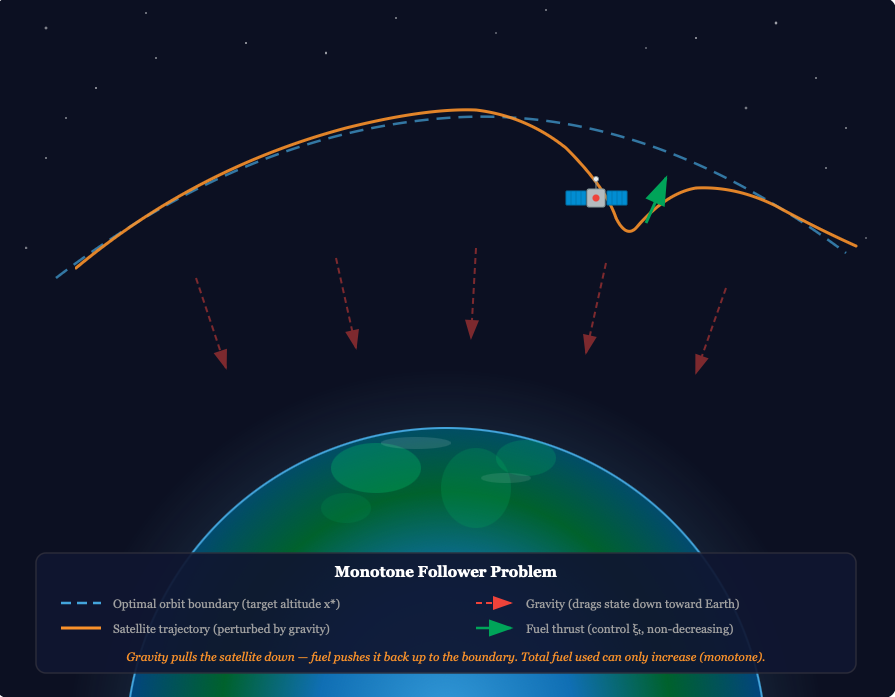
\includegraphics[width=0.6\textwidth]{image.png}
  \end{figure}
\end{frame}


% Upload the stefan_frames/ folder to your Overleaf project, then:
\begin{frame}{Stefan Problem: Ice Melting}
  \begin{figure}
    \centering
    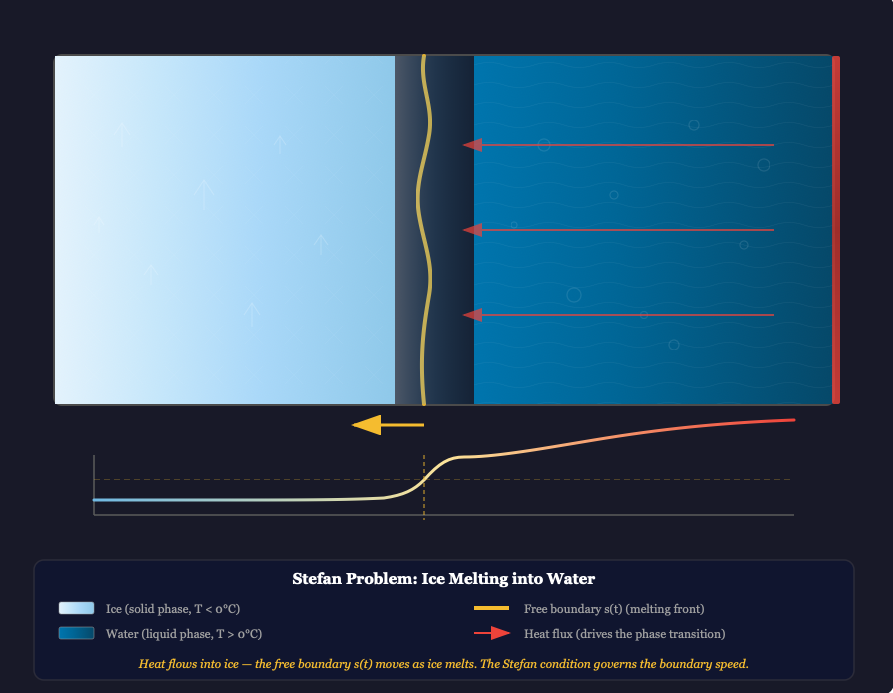
\includegraphics[width=0.55\textwidth]{imagecopy.png}
    \caption{The free boundary $s(t)$ advances as heat melts ice into water.
    \href{run:stefan_animation.html}{\textcolor{blue}{[Click for animation]}}}
  \end{figure}
\end{frame}



\begin{frame}{What Is the Monotone Follower Problem?}
  \begin{itemize}
    \item A \textbf{stochastic control} problem where the controller
          chooses a \emph{non-decreasing}, adapted process~$\xi = \{\xi_t\}_{t\ge 0}$.
    \item The state evolves as
    \[
      X_t = x + \int_0^t b(X_s)\,\df s
            + \int_0^t \sigma(X_s)\,\df W_s + \xi_t,
    \]
    where $W$ is a standard Brownian motion.
    \item The controller seeks to \textbf{minimise} a cost functional that
          balances a running cost against the cumulative cost of intervention:
          \begin{equation*}
            J(x;\xi) = \inf_{\xi}\E_x\!\left[
              \int_0^{T} \, f(X_t)\,\df t + \hat{\xi}_T
            \right].
          \end{equation*}
  \item where $\hat{\xi}_T=\xi^+_T+\xi^-_T$ is the net control applied up to time $T$.
  \end{itemize}
\end{frame}


% ----------------------------------------------------------
\begin{frame}{Historical Context}
  \begin{itemize}
    \item \textbf{Bather \& Chernoff (1967a, 1967b):}
          Early formulation as a sequential decision problem (finite-fuel spaceship control).
    \item \textbf{Bene\v{s}, Shepp \& Witsenhausen (1980):}
          Explicit solutions for several singular control problems.
    \item \textbf{Karatzas (1981):}
          Monotone follower formulation and reduction to a free-boundary problem.
    \item \textbf{Karatzas (1983):}
          A class of singular stochastic control problems.
    \item \textbf{Karatzas \& Shreve (1984):}
          Connection between optimal stopping and singular stochastic control.
    \item \textbf{El Karoui \& Karatzas (1988):}
          General existence results via convex duality.
    \item Modern extensions: multi-dimensional controls, regime switching,
          mean-field interactions, L\'evy-driven dynamics.
  \end{itemize}
\end{frame}

% ----------------------------------------------------------
\begin{frame}{Motivating Applications}
  \begin{columns}[T]
    \column{0.48\textwidth}
    \textbf{Economics \& Finance}
    \begin{itemize}
      \item Irreversible investment under uncertainty
      \item Optimal dividend policy
      \item Inventory management
      \item Real options with sunk costs
    \end{itemize}

    \column{0.48\textwidth}
    \textbf{Engineering \& Operations}
    \begin{itemize}
      \item Spacecraft fuel-optimal attitude control
      \item Dam and reservoir management
      \item Queueing system regulation
      \item Tracking a stochastic signal
    \end{itemize}
  \end{columns}
\end{frame}

\begin{frame}{A solvable example}
\begin{itemize}
\item We first study the work in \cite{BSW1980}.
\item Authors want to solve the following problem:
\begin{equation*}
\inf_{\xi \in \Xi} \mathbb{E} \Bigg[ \int_0^T (x + W_t - \xi_t)^2 \, dt \Bigg]
\end{equation*}
where the class of controls $\Xi$ is given by
\begin{equation*}
\Xi = \left\{ \xi : 
\begin{array}{l}
\xi \text{ is adapted to } (x,W), \\
\xi_0 = 0, \\
\theta_0 \le \xi_t \le \theta_1
\end{array}
\right\}.
\end{equation*}
\item A closed-form solution is obtained $\theta_0=0$, $\theta_1=\infty$.
\end{itemize}
\end{frame}

\begin{frame}
  \begin{itemize}
    \item The \textcolor{red}{Bellman} (HJB) equation which solution $v$ is defined as
    \begin{equation*}
      v(\tau,x)= \inf_{\xi \in \Xi} \mathbb{E} \Bigg[ \int_{T-\tau}^T (x_t)^2 \mathrm{d}t \Bigg | x_{T-\tau }0=x \Bigg].
    \end{equation*}
    is given by 
    \begin{equation*}
      v_t = x^2 + \frac{1}{2}v_{xx}+\inf_{0\leq u \leq \infty} (- u v_x)
    \end{equation*}
    See that $v_x \leq 0$ 
    \begin{equation*}
      \begin{cases}
        v_x < 0 \implies u^* = 0, \quad \text{not exercising zone}\\ 
        v_x = 0 \implies u^* \in [0,\infty), \quad \text{exercise zone} 
      \end{cases}
    \end{equation*}
  \end{itemize}
\end{frame}


\begin{frame}
  \begin{itemize}
    \item The problem is then to vind the couple of functions $(v, f(\tau))$ that solve the PDE
    \begin{equation*}
      \begin{cases}
        v_t = x^2 + \frac{1}{2}v_{xx}, \quad x < f(\tau)\\ 
        v_x = 0, \quad x \geq f(\tau) 
      \end{cases}
    \end{equation*}
    \item The solution can be found by a scaling argument. 
    \item See that since $W_s \sim \square \tau W_s
  \end{itemize}
\end{frame}

% ----------------------------------------------------------
\begin{frame}{Numerical Methods}
  \begin{table}[h]
    \centering
    \renewcommand{\arraystretch}{1.3}
    \begin{tabular}{@{}lll@{}}
      \toprule
      \textbf{Method} & \textbf{Approach} & \textbf{Key Reference} \\
      \midrule
      Finite differences & Discretise HJB / VI & Kushner \& Dupuis (2001) \\
      Penalty method     & Approximate $\xi$ by
                           $\varepsilon^{-1}$ terms & Lions \& Sznitman (1984) \\
      Policy iteration   & Iterate on free boundary & Huang \& Forsyth (2012) \\
      Monte Carlo        & Regression-based
                           (Longstaff--Schwartz) & Belomestny et al.\ (2015) \\
      Deep learning      & Neural net for $V$ or $\xi^*$ & Han et al.\ (2018) \\
      \bottomrule
    \end{tabular}
  \end{table}

  \begin{itemize}
    \item Curse of dimensionality is severe for $d \ge 3$.
    \item Deep learning approaches scale better but lack convergence guarantees.
  \end{itemize}
\end{frame}

% ============================================================
\section{Summary \& Open Problems}
% ============================================================

\begin{frame}{Summary}
  \begin{enumerate}
    \item The \textbf{monotone follower} is a canonical singular stochastic
          control problem with wide applicability.
    \item The value function satisfies a \textbf{variational inequality}
          with free-boundary structure.
    \item A powerful \textbf{duality} links singular control to optimal stopping
          via differentiation of the value function.
    \item Explicit solutions exist in the linear--quadratic Gaussian case
          (Skorokhod reflection at $x^*$).
    \item Extensions to multi-dimensional, L\'evy, and mean-field settings
          remain active research areas.
  \end{enumerate}
\end{frame}

% ----------------------------------------------------------
\begin{frame}{Open Problems}
  \begin{itemize}
    \item \textbf{Regularity of the free boundary} in multi-dimensional
          singular control.
    \item \textbf{Non-convex running costs:} breakdown of the classical
          smooth-fit approach.
    \item \textbf{Model uncertainty / robustness:}
          minimax monotone follower under ambiguity.
    \item \textbf{Mean-field games} with singular controls:
          existence and uniqueness of Nash equilibria.
    \item \textbf{Data-driven approaches:} reinforcement learning for
          singular control without model knowledge.
  \end{itemize}
\end{frame}

% ============================================================
\section*{References}
% ============================================================

\begin{frame}[allowframebreaks]{References}
  \small
  \begin{thebibliography}{99}
    \bibitem{BC1967a}
    J.A.~Bather, H.~Chernoff,
    \emph{Sequential decisions in the control of a spaceship},
    in: Proc.\ Fifth Berkeley Symp.\ Math.\ Statist.\ Probab., Vol.~3,
    Univ.\ California Press (1967), 181--207.

    \bibitem{BC1967b}
    J.A.~Bather, H.~Chernoff,
    \emph{Sequential decisions in the control of a space-ship (finite fuel)},
    J.~Appl.\ Probab.\ \textbf{4} (1967), 584--604.

    \bibitem{BSW1980}
    V.E.~Bene\v{s}, L.A.~Shepp, H.S.~Witsenhausen,
    \emph{Some solvable stochastic control problems},
    Stochastics \textbf{4} (1980), 39--83.

    \bibitem{K1981}
    I.~Karatzas,
    \emph{The monotone follower problem in stochastic decision theory},
    Appl.\ Math.\ Optim.\ \textbf{7} (1981), 179--194.

    \bibitem{K1983}
    I.~Karatzas,
    \emph{A class of singular stochastic control problems},
    Adv.\ Appl.\ Probab.\ \textbf{15} (1983), 225--254.

    \bibitem{KS1984}
    I.~Karatzas, S.E.~Shreve,
    \emph{Connections between optimal stopping and singular stochastic control~I: Monotone follower problems},
    SIAM J.~Control Optim.\ \textbf{22} (1984), 856--877.

    \bibitem{EKK1988}
    N.~El~Karoui, I.~Karatzas,
    \emph{Probabilistic aspects of finite-fuel, reflected follower problems},
    Acta Appl.\ Math.\ \textbf{11} (1988), 223--258.

    \bibitem{KD2001}
    H.J.~Kushner, P.~Dupuis,
    \emph{Numerical Methods for Stochastic Control Problems in Continuous Time},
    Springer, 2nd ed., 2001.

    \bibitem{PS2006}
    G.~Peskir, A.~Shiryaev,
    \emph{Optimal Stopping and Free-Boundary Problems},
    Birkh\"auser, 2006.

    \bibitem{FS2006}
    W.H.~Fleming, H.M.~Soner,
    \emph{Controlled Markov Processes and Viscosity Solutions},
    Springer, 2nd ed., 2006.

    \bibitem{BCZ2017}
    E.~Bayraktar, T.~Cai, Z.~Zhang,
    \emph{On the monotone follower problem in mean-field game theory},
    Preprint, 2017.
  \end{thebibliography}
\end{frame}

% ------ Thank You ------
\begin{frame}
  \centering
  \vspace{1.5cm}
  {\Huge\bfseries Thank You!}

  \vspace{1cm}
  {\large Questions \& Discussion}

  \vspace{1cm}
  {\normalsize \texttt{your.email@university.edu}}
\end{frame}

\end{document}